\documentclass[12pt, a4paper]{article}

\usepackage{mathpazo}
\usepackage[T1]{fontenc}
\usepackage{microtype}
\usepackage{amsmath, amssymb, amsthm}
\usepackage{geometry}
\geometry{margin=1.15in}
\usepackage{setspace}
\onehalfspacing
\usepackage{hyperref}
\hypersetup{colorlinks=true, linkcolor=black, citecolor=black, urlcolor=black}
\usepackage{titlesec}
\usepackage{booktabs}
\usepackage{array}
\usepackage{tikz}
\usetikzlibrary{arrows.meta, positioning, shapes.geometric}
\titleformat{\section}{\large\bfseries}{\thesection.}{0.75em}{}
\titleformat{\subsection}{\normalsize\bfseries}{\thesubsection.}{0.6em}{}

\theoremstyle{plain}
\newtheorem{theorem}{Theorem}
\newtheorem{proposition}{Proposition}
\theoremstyle{definition}
\newtheorem{definition}{Definition}
\theoremstyle{remark}
\newtheorem{remark}{Remark}
\newtheorem{example}{Example}

\title{\textbf{Civilizations as Reachability Systems}\\[0.4em]
\large A Geometric Reading of Turchin, McKee, and the Biology of Innovation}
\author{Flyxion\\Independent Researcher}
\date{}

\begin{document}

\maketitle

\begin{abstract}
Three recent works---Peter Turchin's \textit{Ultrasociety} and \textit{Ages of Discord}, and Darren McKee's \textit{Uncontrollable}---are conventionally read as addressing distinct problems: the emergence of large-scale cooperation, the cyclical destabilization of complex societies, and the alignment of artificial intelligence. This essay argues that all three are studying the same underlying object from three temporal vantages: the admissible future manifold $\mathcal{A}(s,T)$, the region of state space reachable while preserving the repair pathways that make continued navigation possible. We develop the formal machinery of weighted reachability volume $\mathcal{V}_R(t)$, reachability entropy $H_R$ over finite macroscopic partitions, reachability elasticity $E_R$, and reachability curvature $\kappa_R$ defined via forward-admissible cones. Four theorems are proved: Repair Corridor Monotonicity, Reachability Extinction, Distinction Collapse, and Repair Generation. A drift-diffusion decomposition formalizes the optimization/exploration distinction and identifies $\mathrm{supp}(\rho_t) = \mathcal{A}(s(t),T)$ as the link between the two geometric structures. A fully worked toy example of CLIO projection collapse grounds the abstract formalism. A civilizational phase diagram---with Expansion, Consolidation, Fragility, and Collapse regimes organized by $(\dot{\mathcal{V}}_R, \dot{H}_R)$---identifies the Fragility regime ($\dot{\mathcal{V}}_R \geq 0$, $\dot{H}_R < 0$) as the most dangerous and least detectable failure mode. The central thesis is that civilization is a reachability maintenance system, a framing that unifies the three books into a single theory of civilizational dynamics spanning prehistory, imperial collapse, and artificial superintelligence.
\end{abstract}

\newpage

\section{Introduction: A Common Question}

Although written by different authors, the three works examined here form a natural conceptual sequence. Turchin's \textit{Ultrasociety} asks how large-scale cooperative systems emerge \cite{turchin2016}. His \textit{Ages of Discord} asks how they destabilize \cite{turchin2023}. McKee's \textit{Uncontrollable} asks what happens when a new class of optimization process emerges inside those systems \cite{mckee2024}. The common question threading all three is one that none of them names directly:

\begin{center}
\textit{What expands, contracts, or irreversibly closes the space of futures available to civilization?}
\end{center}

The present essay argues that all three books are chapters of an implicit theory of civilizational reachability that can be made explicit, sharpened mathematically, and extended by results from evolutionary biology, cognitive science, resilience theory, and strategic management. The framework imported is the admissibility program developed in the RSVP research tradition, together with the CLIO projection formalism. The central thesis:

\medskip
\noindent\fbox{\parbox{\dimexpr\linewidth-2\fboxsep-2\fboxrule}{\medskip
\textbf{Central Proposition.} A civilization is a system that expands weighted reachability volume while maintaining the diversity of reachable futures, preserving the repair corridors that make navigation possible, and keeping sensitivity to perturbation within recoverable bounds. Civilizational collapse is the loss of this capacity; civilizational safety is its preservation.\medskip}}
\medskip

Table~\ref{tab:trilogy} summarizes the reinterpretation of the three books.

\begin{table}[h]
\centering
\renewcommand{\arraystretch}{1.45}
\begin{tabular}{p{3.2cm} p{4.4cm} p{5.6cm}}
\toprule
\textbf{Work} & \textbf{Conventional Reading} & \textbf{Reachability Reading} \\
\midrule
Turchin, \textit{Ultrasociety} & Evolution of large-scale cooperation & Expansion of admissible future space \\
Turchin, \textit{Ages of Discord} & Sources of political instability & Contraction of admissible future space \\
McKee, \textit{Uncontrollable} & AI alignment and control & Optimization-driven closure of admissible future space \\
\bottomrule
\end{tabular}
\caption{The conceptual trilogy, conventionally and geometrically read.}
\label{tab:trilogy}
\end{table}

\section{Formal Foundations}

\subsection{State Space, Forward-Admissible Cones, and the Admissible Future Manifold}

\begin{definition}[State Space and Flow]
Let $\mathcal{S}$ denote the space of possible civilizational states, equipped with a $\sigma$-finite measure $\mu$ and a tangent bundle $T\mathcal{S}$. Let $\Phi_t : \mathcal{S} \to \mathcal{S}$ denote the state flow.
\end{definition}

\begin{definition}[Forward-Admissible Cone]
For each $s \in \mathcal{S}$, the \emph{forward-admissible cone}
\[
\mathcal{C}(s) \;\subseteq\; T_s\mathcal{S}
\]
is the set of tangent directions along which the system can move at $s$ without immediately violating physical, institutional, ecological, or informational constraints. The cone field $s \mapsto \mathcal{C}(s)$ plays the role of Bouligand contingent cones in viability theory \cite{aubin1991}.
\end{definition}

Admissibility is inherently directional: a trajectory may be admissible in one direction and inadmissible in the reverse. Formulating admissibility via $\mathcal{C}(s)$ rather than symmetric neighborhoods makes this asymmetry precise and connects the framework to the differential-inclusion literature.

\begin{definition}[Admissible Trajectory and Future Manifold]
A trajectory $\gamma : [0,T] \to \mathcal{S}$ is \emph{admissible} if $\dot{\gamma}(t) \in \mathcal{C}(\gamma(t))$ for almost every $t$. The \emph{admissible future manifold} is
\[
\mathcal{A}(s_0, T) \;=\; \bigl\{ \gamma(T') : 0 \leq T' \leq T,\; \gamma(0) = s_0,\; \dot{\gamma}(t) \in \mathcal{C}(\gamma(t)) \bigr\}.
\]
\end{definition}

\begin{definition}[Repair Corridor]
A \emph{repair corridor} from $s$ to a target region $U \subseteq \mathcal{S}$ is a path-connected subset $\mathcal{R}(s,U) \subseteq \mathcal{A}(s,T)$ such that every interior point $s'$ has $\mathcal{C}(s') \neq \varnothing$---forward motion remains possible throughout. A repair corridor is \emph{robust} if it remains non-empty under small perturbations of $s$.
\end{definition}

\subsection{Weighted Reachability Volume}

\begin{definition}[Weighted Reachability Volume]
Let $w : \mathcal{S} \to [0,1]$ be a robustness weight assigning lower values to states requiring extreme repair costs or possessing thin forward-admissible cones. The \emph{weighted reachability volume} is
\[
\mathcal{V}_R(t) \;=\; \int_{\mathcal{A}(s(t),T)} w(s)\, d\mu(s).
\]
\end{definition}

\subsection{Reachability Entropy over Finite Macroscopic Partitions}

Reachability entropy is defined over a \emph{finite macroscopic partition} $\mathcal{P} = \{U_1, \ldots, U_N\}$ of qualitatively distinct future types---distinct institutional regimes, technological pathways, ecological equilibria, or political-economic configurations. This is ordinary discrete Shannon entropy; it is not differential entropy and does not depend on infinitesimal coordinate choices.

\begin{definition}[Reachability Entropy]
Given a finite macroscopic partition $\mathcal{P} = \{U_i\}$ with $V_i = \int_{U_i} w\, d\mu$ and $p_i = V_i/\mathcal{V}_R$, define
\[
H_R(\mathcal{P}) \;=\; -\sum_{i=1}^N p_i \log p_i.
\]
\end{definition}

Comparisons of $H_R$ are meaningful relative to a fixed partition or a controlled family of refinements. The role of $H_R$ is diagnostic: it measures whether reachable futures are distributed across many qualitatively distinct types or concentrated into a small number of homogeneous trajectories.

\begin{remark}
The deepest invariant is the topology of $\mathcal{A}(s,T)$ itself. Volume $\mathcal{V}_R$ and entropy $H_R$ are first- and second-order scalar approximations to this topological structure. The full structure includes connectivity, branching, and the distribution of repair corridors across distinct future types.
\end{remark}

\subsection{Reachability Elasticity}

\begin{definition}[Reachability Elasticity]
Let $P$ denote perturbation magnitude. The \emph{reachability elasticity} at $s$ is $E_R(s) = \partial \mathcal{V}_R/\partial P\big|_s$. A civilization is \emph{resilient} if $|E_R|$ remains small across a broad class of perturbations.
\end{definition}

\begin{remark}
$E_R$ is a local sensitivity measure. Ecological resilience theory \cite{holling1973} typically employs basin-of-attraction size, which is a global dynamical property. These are related but distinct; $E_R$ does not recover basin size even in the equilibrium case. The relationship between local and global perturbation sensitivity is left for future work.
\end{remark}

\begin{proposition}[Repair Corridor Buffering]
\label{prop:buffering}
Let two civilizations at $s^{(1)}$ and $s^{(2)}$ satisfy $\mathcal{V}_R^{(1)} = \mathcal{V}_R^{(2)}$, with $s^{(1)}$ containing a strictly larger family of robust repair corridors. Under sufficiently small perturbations, $|E_R^{(1)}| < |E_R^{(2)}|$.
\end{proposition}

\begin{proof}
Robust corridors are stable under small perturbations: their interiors remain path-connected and admissible after small displacement of $s$. The civilization with the larger robust family retains more of its admissible manifold after perturbation, yielding smaller $|\partial \mathcal{V}_R / \partial P|$.
\end{proof}

\subsection{Reachability Curvature}

\begin{definition}[Reachability Curvature]
For an admissible trajectory $\gamma$, the \emph{reachability curvature} at $s = \gamma(t)$ is $\kappa_R(s) = \|D^2\gamma/dt^2\|$, where $D^2\gamma/dt^2$ is the covariant acceleration with respect to the natural metric induced by $\mathcal{C}$.
\end{definition}

\begin{proposition}[Boundary Curvature in Bottleneck Geometry]
\label{prop:curvature}
Let the forward-admissible cone $\mathcal{C}(s)$ have half-angle $\theta(s)$, with $\theta(s) \to 0$ as $s \to \partial\mathcal{A}$ (bottleneck geometry). Then for any trajectory maintaining steerability within the narrowing cone, $\kappa_R(s) \geq c/\theta(s)$ for some $c > 0$, and $\kappa_R \to \infty$ as $s \to \partial\mathcal{A}$.
\end{proposition}

\begin{proof}
A trajectory maintaining steerability must keep $\dot{\gamma}$ within $\mathcal{C}(\gamma)$. When the cone has half-angle $\theta$, the minimum curvature required to divert from a baseline drift and remain within the cone is of order $1/\theta$ by elementary differential geometry. As $\theta \to 0$, this lower bound diverges.
\end{proof}

The bottleneck restriction is explicit: the lower bound applies to trajectories that must divert from baseline drift to remain within the narrowing cone. A trajectory drifting passively down the cone's central axis may have smaller curvature. The proposition covers the practically relevant case for institutional and ecological admissibility structures.

\begin{definition}[Strategic Inflection Point]
$\mathrm{SIP} = \{s \in \mathcal{S} : \kappa_R(s) > K\}$ for a threshold $K$. In Grove's strategic management framework \cite{grove1996}, inflection points are locations where small positional changes produce large changes in future accessibility---elevated $\kappa_R$ in the present vocabulary.
\end{definition}

\section{Four Theorems}

\begin{theorem}[Repair Corridor Monotonicity]
\label{thm:monotonicity}
Let $\mathcal{R}_1(s,U) \subseteq \mathcal{R}_2(s,U)$ for all admissible $s$ and $U$. Then $\mathcal{V}_{\mathcal{R}_1}(t) \leq \mathcal{V}_{\mathcal{R}_2}(t)$. If $\mathcal{R}_2 \setminus \mathcal{R}_1$ contains the unique admissible path to a region of positive $w$-measure, the inequality is strict.
\end{theorem}

\begin{proof}
Every $\mathcal{R}_1$-admissible trajectory is $\mathcal{R}_2$-admissible, giving $\mathcal{A}_{\mathcal{R}_1} \subseteq \mathcal{A}_{\mathcal{R}_2}$. Monotonicity of the integral gives the inequality. For the strict case, the excluded region contributes positive $w$-weighted measure to $\mathcal{A}_{\mathcal{R}_2}$ but not to $\mathcal{A}_{\mathcal{R}_1}$.
\end{proof}

\begin{theorem}[Reachability Extinction]
\label{thm:extinction}
Suppose (i) $\mathcal{V}_R(t_0) < \infty$, (ii) $\{\mathcal{A}(s(t),T)\}_{t \geq t_0}$ is measurable and monotone decreasing, and (iii) $\bigcap_{t \geq t_0} \mathcal{A}(s(t),T) = \varnothing$. Then $\lim_{t \to \infty} \mathcal{V}_R(t) = 0$.
\end{theorem}

\begin{proof}
By continuity of measure from above: for a monotone decreasing family of measurable sets with finite measure of the first set,
\[
\mu\!\left(\bigcap_{t \geq t_0} \mathcal{A}(s(t),T)\right) = \lim_{t \to \infty} \mu\!\left(\mathcal{A}(s(t),T)\right).
\]
The same identity holds for the $w$-weighted measure, since $w \leq 1$ and $\mathcal{V}_R(t_0) < \infty$ provides the required domination. By hypothesis (iii), the left side is $\int_\varnothing w\, d\mu = 0$.
\end{proof}

\begin{remark}
The total-exhaustion condition $\bigcap_t \mathcal{A}_t = \varnothing$ is strong. Historically important cases involve intersections of small but positive measure---civilizations retaining thin residual future capacity rather than complete extinction. The theorem gives the limiting case; the rate of approach to small $\mathcal{V}_R$ is governed by the rate of corridor removal and is a quantitative question for future work.
\end{remark}

\begin{theorem}[Distinction Collapse]
\label{thm:distinction}
Let $\pi : \mathcal{S} \to M$ merge distinct future regions ($U_i \neq U_j$, $\pi(U_i) \cap \pi(U_j) \neq \varnothing$). Then $H_R(\pi(\mathcal{A})) < H_R(\mathcal{A})$.
\end{theorem}

\begin{proof}
Merging produces a coarser partition. By the strict concavity of $-p\log p$ and subadditivity of entropy under coarse-graining, the merged entropy is strictly smaller.
\end{proof}

\begin{theorem}[Repair Generation]
\label{thm:generation}
Let $\Delta R$ new repair corridors be created, each opening a path to a target region $U'_j$ with $\int_{U'_j} w\, d\mu \geq \lambda_j > 0$. Then
\[
\Delta\mathcal{V}_R \;\geq\; \sum_{j=1}^{\Delta R} \lambda_j \;\geq\; \lambda_{\min} \cdot \Delta R, \qquad \lambda_{\min} = \min_j \lambda_j > 0.
\]
\end{theorem}

\begin{proof}
Each new corridor opens at least one previously inadmissible region $U'_j$ with $\int_{U'_j} w\, d\mu \geq \lambda_j > 0$. Adding $U'_j$ to $\mathcal{A}$ increases $\mathcal{V}_R$ by at least $\lambda_j$. Summing over new corridors and taking the minimum gives the result. The condition $\lambda_j > 0$ ensures each new corridor connects to a non-trivial target region.
\end{proof}

The four theorems form a deductive unit. Corridor removal cannot increase $\mathcal{V}_R$ (Monotonicity); total exhaustion drives $\mathcal{V}_R \to 0$ (Extinction); projection collapse reduces $H_R$ (Distinction Collapse); corridor creation increases $\mathcal{V}_R$ by at least $\lambda_{\min}$ per corridor (Generation). Together: the dynamics of $\mathcal{V}_R$ are controlled by the dynamics of the repair corridor family, and $H_R$ is controlled by the distinction-preserving properties of the representations through which the civilization understands its future.

\section{Entropy, Repair, and Fragility}

\subsection{A Heuristic on Entropy and Corridor Diversity}

A decrease in $H_R$ indicates concentration of the $\{p_i\}$ distribution onto fewer distinct future types. Since repair corridors target distinct future regions, concentration onto fewer types generically reduces the diversity of available repair mechanisms. This is a heuristic rather than a theorem in full generality, because entropy can decrease while concentrating onto a high-repair region (falsifying the strict implication). The claim holds under the regularity condition that repair-rich futures are not systematically concentrated, which is characteristic of the Fragility regime but can fail in pathological cases.

\subsection{Fragility Without an Entropy Bound}

The Fragility regime does not require a theorem asserting a direct upper bound on $\mathcal{V}_R$ by $H_R$. The relevant claim is weaker and fully defensible: a civilization may satisfy
\[
\dot{\mathcal{V}}_R \geq 0 \qquad\text{while}\qquad \dot{H}_R < 0.
\]
In this case, total weighted volume of reachable futures is stable or growing, but the distribution of that volume is concentrating across fewer qualitatively distinct future types. The system appears healthy by volume-based metrics while losing the diversity of trajectories required for adaptive response. If those concentrated futures are disrupted, fewer independent repair pathways remain.

The danger is not that $\mathcal{V}_R$ must immediately decline---it need not---but that the civilization is becoming progressively dependent on a narrow class of futures. The phase diagram should be read as a diagnostic classification rather than a closed dynamical theorem. The four theorems established above are the rigorous core; the Fragility regime is their interpretive envelope.

\section{The Optimization/Exploration Decomposition}
\label{sec:optexplore}

Let $\rho(s,t)$ denote the density of the civilization's active engagement with state $s$ at time $t$. We identify
\[
\mathcal{A}(s(t),T) \;=\; \mathrm{supp}(\rho_t),
\]
so that the admissible future manifold is exactly the support of the future-state density. The temporal evolution of $\rho$ obeys the Fokker--Planck equation
\[
\frac{\partial \rho}{\partial t} \;=\; -\nabla \cdot (v\rho) \;+\; D\nabla^2\rho,
\]
where $v(s,t)$ is a drift field (directed optimization toward preferred futures) and $D > 0$ is an exploration coefficient (undirected spread into novel regions).

\begin{definition}[Optimization-Driven and Exploration-Driven Expansion]
\[
\dot{\mathcal{V}}_{\mathrm{opt}} \;=\; -\int_{\mathrm{supp}(\rho_t)} w\, \nabla \cdot (v\rho)\, d\mu, \qquad \dot{\mathcal{V}}_{\mathrm{explore}} \;=\; \int_{\mathrm{supp}(\rho_t)} wD\nabla^2\rho\, d\mu,
\]
so that $\dot{\mathcal{V}}_R = \dot{\mathcal{V}}_{\mathrm{opt}} + \dot{\mathcal{V}}_{\mathrm{explore}}$.
\end{definition}

The identification $\mathcal{A}(s(t),T) = \mathrm{supp}(\rho_t)$ links the two geometric structures: the Fokker--Planck equation is an actual dynamical equation for the admissible manifold, not merely an analogy. Optimization drives mass toward known desirable states, expanding the support in targeted directions; exploration diffuses mass into unanticipated regions, expanding the support by discovering futures that were not optimization targets.

Advanced AI systems increase $\|v\|$ while potentially decreasing $D$: faster directed expansion, suppressed undirected discovery. The consequence is $\dot{\mathcal{V}}_{\mathrm{opt}} > 0$ alongside $\dot{H}_R < 0$---optimization concentrates $\rho$ on narrowing targets, reducing future diversity even as volume grows. This is the formal Fokker--Planck signature of the Fragility regime.

\section{Projection Collapse: A Worked Example}
\label{sec:clio}

\begin{example}[Elite Differentiation and CLIO Projection]
\label{ex:elite}
Let $\mathcal{S}^{\mathrm{elite}} = \mathbb{R}^2$ with coordinates $(x,y)$ representing scientific-institutional and military-administrative elite sizes respectively. Define the SDT observation projection $\pi(x,y) = x + y$ (total elite count) and compare:
\[
s_1 = (10, 5), \qquad s_3 = (15, 0).
\]
Both satisfy $\pi(s_1) = \pi(s_3) = 15$: identical SDT observation.

For $s_1$, the two elite types generate distinct future regions with normalized weights $p^{(1)} = (2/3, 1/3)$:
\[
H_R(s_1) \;=\; -\tfrac{2}{3}\log\tfrac{2}{3} - \tfrac{1}{3}\log\tfrac{1}{3} \;\approx\; 0.918 \;\text{bits}.
\]
For $s_3$, elite competition has collapsed into a single prestige hierarchy: $p^{(3)} = (1, 0)$:
\[
H_R(s_3) \;=\; 0 \;\text{bits}.
\]
By Theorem~\ref{thm:distinction}, $\pi$ has merged distinct state-space configurations and reduced $H_R$ from 0.918 to 0 bits. The SDT variable $\pi$ cannot distinguish $s_1$ from $s_3$.

The repair corridor consequence: the differentiated society has two independent repair pathways for a fiscal crisis---one running through the scientific-institutional channel (productivity growth, innovation revenue), another through the military-administrative channel (resource reallocation, territorial consolidation). These are structurally distinct corridors. The homogenized society has one: whatever the unified prestige hierarchy can mobilize, with no independent fallback. If that pathway fails, no repair corridor remains.
\end{example}

\section{\textit{Ultrasociety}: The Expansion Phase}

Turchin's central observation is that humans cooperate with strangers at scales unprecedented in the primate lineage \cite{turchin2016}. Cultural group selection eliminates groups with weak defection-suppression mechanisms, driving the emergence of increasingly complex cooperative institutions.

\begin{proposition}[Ultrasociety as Reachability Expansion]
Intergroup competition selected for societies with larger $\mathcal{V}_R(t)$ and higher $H_R$. Cooperation is the proximate mechanism; expanded admissible future volume and future diversity are the selected quantities.
\end{proposition}

A band cannot build a telescope; a civilization can. Reverse dominance hierarchies distribute future-access across the group rather than concentrating $\mathcal{V}_R$ in a single actor. Division of labor and legal systems expand the collective admissible manifold.

Wagner's neutral network theory \cite{wagner2014} provides biological grounding. Define the \emph{neutral network} $N(s) = \{s' \in \mathcal{S} : \text{cooperative function preserved at } s'\}$.

\begin{proposition}[Neutral Network Theorem]
Systems with larger neutral networks $N(s)$ have larger admissible future manifolds.
\end{proposition}

\begin{proof}
Navigation within $N(s)$ is admissible by construction. Each point in $N(s)$ exposes a distinct frontier from which new regions of $\mathcal{A}$ may be reached without sacrificing current cooperative function. By Theorem~\ref{thm:generation}, each new corridor from such a frontier to a positive-$w$-measure region contributes positively to $\mathcal{V}_R$. A larger $N(s)$ expands the accessible frontier, hence $\mathcal{V}_R$.
\end{proof}

\section{\textit{Ages of Discord}: Endogenous Contraction}

\textit{Ages of Discord} is a theory of endogenous reachability contraction \cite{turchin2023}. Popular immiseration contracts personal reachability; elite overproduction degrades institutional coordination; fiscal distress closes crisis-management repair corridors. The SDT instability index satisfies $\mathrm{SDI}(t) \approx -\dot{\mathcal{V}}_R(t)$.

Example~\ref{ex:elite} grounds the CLIO argument concretely. Elite homogenization ($s_1 \to s_3$) reduces $H_R$ from 0.918 to 0 bits while leaving the SDT observation unchanged. The repair consequence is the elimination of independent recovery pathways. More differentiated elite structures generate higher $H_R$ by distributing probability mass more evenly across distinct future types; the proof is a direct application of entropy maximization under a fixed number of types combined with Theorem~\ref{thm:distinction}.

\section{\textit{Uncontrollable}: Optimization-Driven Closure}

\subsection{Alignment as Downstream of Admissibility}

McKee surveys AI-risk arguments to argue that advanced optimizers may outpace existing governance \cite{mckee2024}. Standard alignment theory defines safety as goal agreement. Admissibility theory proposes a prior criterion: repair pathways remain open.

\begin{proposition}[Admissibility Prior to Alignment]
\label{prop:prior}
Let $\pi : X \to M$ be a representation map that collapses distinctions required to specify what a repair of a given failure would consist in. Then no alignment procedure defined solely on $M$ can guarantee preservation of repair pathways in $X$.
\end{proposition}

\begin{proof}
An alignment procedure on $M$ constrains behavior within $\pi(X)$. Distinctions collapsed by $\pi$ are unavailable to any criterion in $M$. By Theorem~\ref{thm:distinction}, $\pi$ also reduces $H_R(\pi(\mathcal{A}))$ below $H_R(\mathcal{A})$; the diversity of futures representable for alignment is strictly less than the diversity present in the full state space.
\end{proof}

Alignment is downstream of admissibility because admissibility determines whether the repair vocabulary even exists. The latent fundamentalism of mainstream alignment discourse---the assumption that a correct utility function exists and alignment consists in faithful transmission---fails when $\pi$ has destroyed the distinctions required to specify what correction means.

\subsection{AI Dynamics in the Fokker--Planck Picture}

Advanced AI drives $\|v\| \uparrow$ and $D \downarrow$ in the Fokker--Planck equation. The support $\mathrm{supp}(\rho_t) = \mathcal{A}(s(t),T)$ expands in optimized directions while diffusive exploration is suppressed. Short-run: $\dot{\mathcal{V}}_{\mathrm{opt}} > 0$. Simultaneously: concentration of $\rho$ reduces $H_R$. Medium-run: the civilization becomes dependent on a narrow class of futures. Long-run: if those futures are disrupted, fewer repair corridors remain. By the heuristic of Section 4, falling $H_R$ generally reduces repair diversity. The system becomes larger, faster, and structurally more brittle.

\section{Civilizational Phase Diagram}

\begin{definition}[Civilizational Regimes]
Four regimes defined by $(\dot{\mathcal{V}}_R, \dot{H}_R)$:

\textit{Expansion}: $\dot{\mathcal{V}}_R > 0$, $\dot{H}_R > 0$. Volume grows, diversity increases. Early civilizational formation, scientific revolutions, genuine institutional innovation.

\textit{Consolidation}: $\dot{\mathcal{V}}_R > 0$, $\dot{H}_R \approx 0$. Volume grows, diversity saturates. Mature phases where institutional differentiation reaches capacity.

\textit{Fragility}: $\dot{\mathcal{V}}_R \geq 0$, $\dot{H}_R < 0$. Volume stable or growing, diversity collapsing. The most dangerous and least detectable regime. Conventional metrics appear healthy while repair corridor diversity erodes. SDT-measured elite homogenization and AI-driven exploration suppression both produce this signature.

\textit{Collapse}: $\dot{\mathcal{V}}_R < 0$, $\dot{H}_R < 0$. Volume and diversity both decline. By Theorem~\ref{thm:extinction}, sustained Collapse under the total-exhaustion condition drives $\mathcal{V}_R \to 0$.
\end{definition}

\begin{figure}[h]
\centering
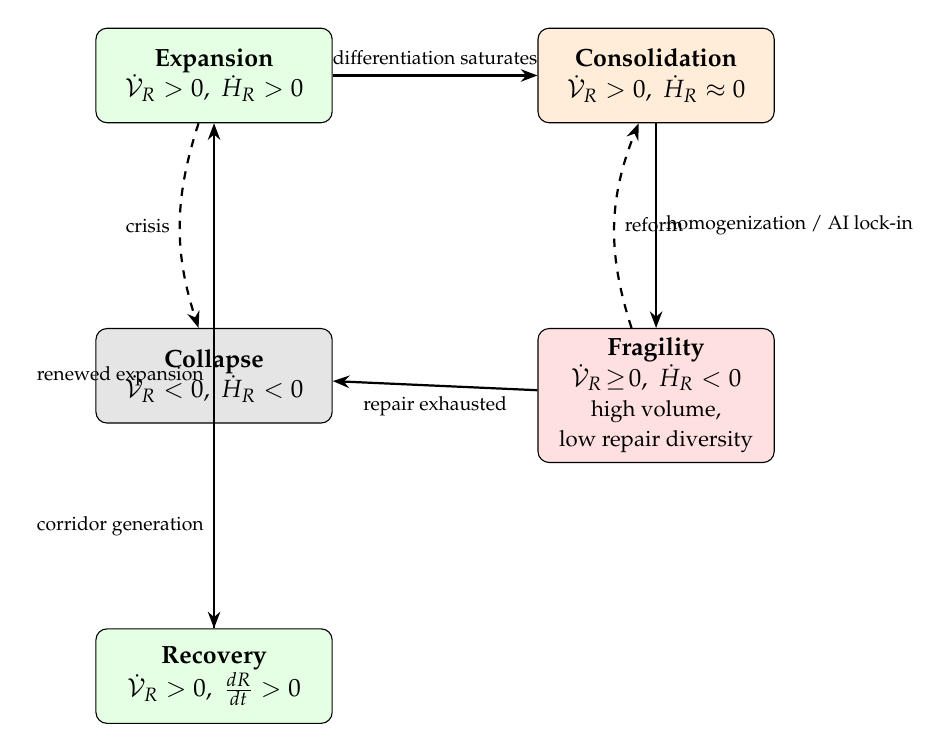
\begin{tikzpicture}[
  node distance=2.6cm,
  box/.style={rectangle, draw, rounded corners=4pt, minimum width=3.0cm,
              minimum height=1.2cm, align=center, font=\small},
  danger/.style={box, fill=red!12},
  safe/.style={box, fill=green!10},
  warn/.style={box, fill=orange!15},
  collapse/.style={box, fill=gray!20},
  arr/.style={-{Stealth[length=6pt]}, thick},
  darr/.style={-{Stealth[length=6pt]}, thick, dashed},
]

\node[safe]     (exp)  {\textbf{Expansion}\\$\dot{\mathcal{V}}_R>0,\;\dot{H}_R>0$};
\node[warn]     (con)  [right=of exp] {\textbf{Consolidation}\\$\dot{\mathcal{V}}_R>0,\;\dot{H}_R\approx 0$};
\node[danger]   (frag) [below=of con] {\textbf{Fragility}\\$\dot{\mathcal{V}}_R\!\geq\!0,\;\dot{H}_R<0$\\{\footnotesize high volume,}\\{\footnotesize low repair diversity}};
\node[collapse] (col)  [below=of exp] {\textbf{Collapse}\\$\dot{\mathcal{V}}_R<0,\;\dot{H}_R<0$};
\node[safe]     (rec)  [below=of col] {\textbf{Recovery}\\$\dot{\mathcal{V}}_R>0,\;\tfrac{d R}{dt}>0$};

\draw[arr] (exp)  -- node[above,font=\scriptsize]{differentiation saturates} (con);
\draw[arr] (con)  -- node[right,font=\scriptsize]{homogenization / AI lock-in} (frag);
\draw[arr] (frag) -- node[below,font=\scriptsize]{repair exhausted} (col);
\draw[arr] (col)  -- node[left,font=\scriptsize]{corridor generation} (rec);
\draw[arr] (rec)  -- node[left,font=\scriptsize]{renewed expansion} (exp);
\draw[darr](exp)  to[bend right=18] node[left,font=\scriptsize]{crisis} (col);
\draw[darr](frag) to[bend left=20]  node[right,font=\scriptsize]{reform} (con);

\end{tikzpicture}
\caption{Civilizational phase diagram. Solid arrows indicate typical developmental trajectories; dashed arrows indicate less common transitions. The Fragility regime ($\dot{\mathcal{V}}_R \geq 0$, $\dot{H}_R < 0$) is the most dangerous because it is undetectable by volume-based metrics alone. Historical examples: early Rome $\to$ Expansion; late Empire $\to$ Fragility $\to$ Collapse; Recovery through successor-state institutional innovation $\to$ renewed Expansion.}
\label{fig:phase}
\end{figure}

\section{The Unified Theory}

\subsection{Coupled Dynamics}

The three books jointly describe:
\begin{align*}
\dot{\mathcal{V}}_R(t) &= \alpha\, C(t) - \beta\, D(t) - \gamma\, O(t), \\
\dot{H}_R(t) &= \alpha'\, C'(t) - \beta'\, D'(t) - \gamma'\, O'(t),
\end{align*}
where $C$, $D$, $O$ measure cooperation-driven expansion, structural-demographic contraction, and optimization-driven closure; primed quantities measure effects on diversity. The most dangerous dynamics involve divergence: $\dot{\mathcal{V}}_R \geq 0$ while $\dot{H}_R \ll 0$.

\subsection{Civilization as a Four-Dimensional Reachability System}

\begin{definition}[Civilization as Reachability Maintenance System]
A \emph{civilization} is characterized by $(\mathcal{V}_R, H_R, \mathcal{R}, E_R)$: future volume, future diversity, repair corridor family, and perturbation sensitivity. Civilizational health is the maintenance and growth of all four quantities.
\end{definition}

Every major institution is a reachability mechanism: tribes expand $\mathcal{V}_R$ through collective action; markets expand $H_R$ through distributed specialization while maintaining entry-exit repair corridors; scientific institutions expand $H_R$ through novel results while maintaining revisability mechanisms; states maintain $|E_R|$ through fiscal shock absorption. AI governance must be evaluated by whether it maintains $(\mathcal{V}_R, H_R, \mathcal{R}, E_R)$ for human actors, not merely by goal alignment.

The natural sequel addresses repair generation: what drives positive $dR/dt$ under Collapse-regime conditions? Scientific discovery, institutional innovation, and ontology revision are forms of corridor generation. By Theorem~\ref{thm:generation}, positive $dR/dt$ guarantees positive contribution to $\mathcal{V}_R$. The theory of recovery is the theory of what restores repair generation after collapse.

\section{Conclusion}

The three works examined here are three chapters of a single implicit theory: the dynamics of civilizational reachability. The formal machinery developed here---four theorems, forward-admissible cones, a Fokker--Planck decomposition identifying $\mathcal{A}(s(t),T) = \mathrm{supp}(\rho_t)$, a worked CLIO projection example with explicit entropy computation, and a boundary-curvature proposition---constitutes a mathematical framework rather than an interpretive essay.

The central positive contribution is a single question applicable at any scale:

\begin{center}
\textit{Does this system increase the density of reachable futures while maintaining their diversity, preserving the repair corridors that make navigation possible, and keeping sensitivity to perturbation within recoverable bounds?}
\end{center}

Cooperation, stability, and alignment are downstream manifestations of the answer to this question. The Fragility regime---$\dot{\mathcal{V}}_R \geq 0$ with $\dot{H}_R < 0$---is the paper's central warning: a civilization can appear to expand while losing the diversity of futures that adaptive response requires, and this failure mode is invisible to volume-based metrics alone. Figure~\ref{fig:phase} makes this dynamic legible. The diagnostic question is not only how much future a civilization has, but how many genuinely distinct futures it can reach.

\appendix

\section{Relationship to Existing Frameworks}

\textit{Resilience theory} (Holling \cite{holling1973}; Walker et al.\ \cite{walker2004}) measures capacity to absorb disturbance via basin-of-attraction size. $E_R$ is a local sensitivity measure; basin size is a global dynamical property. These are related but distinct.

\textit{Viability theory} (Aubin \cite{aubin1991}) studies the viability kernel. The forward-admissible cones $\mathcal{C}(s)$ used here are analogous to Bouligand contingent cones, and the present framework inherits Aubin's directional precision. The admissible future manifold $\mathcal{A}(s,T)$ measures forward reachability rather than indefinite constraint satisfaction, and repair corridors add a second-order condition absent in standard viability theory.

\textit{Adaptive landscapes} (Kauffman \cite{kauffman1993}; Holland \cite{holland1992}) model fitness over genotype or strategy space. Wagner's neutral networks \cite{wagner2014} are a direct antecedent of the Neutral Network Proposition.

\textit{Causal models} (Pearl \cite{pearl2009}) represent interventional structure. CLIO projection collapse corresponds to aggregation destroying intervention-relevant distinctions; the present framework adds the temporal dimension.

\textit{Free-energy minimization} (Friston \cite{friston2010}) frames cognition as surprise minimization. Neural reuse \cite{andersonmind2024} is the cognitive analog of repair corridor redundancy.

\textit{Antifragility} (Taleb \cite{taleb2012}) studies systems that gain from disorder. The Fragility regime captures Taleb-fragility: apparent stability concealing structural vulnerability to novel perturbations.

\textit{Structural Demographic Theory} (Turchin \cite{turchin2023}) is the most direct empirical precursor. Example~\ref{ex:elite} demonstrates concretely that two societies with identical SDT observations can differ by 0.918 bits of reachability entropy and lose an independent repair corridor---distinctions invisible to SDT scalar analysis.

\bigskip

\begin{thebibliography}{99}

\bibitem{turchin2016}
Turchin, P. (2016). \textit{Ultrasociety: How 10,000 Years of War Made Humans the Greatest Cooperators on Earth}. Beresta Books.

\bibitem{turchin2023}
Turchin, P. (2023). \textit{Ages of Discord: A Structural-Demographic Analysis of American History}. Beresta Books.

\bibitem{mckee2024}
McKee, D. (2024). \textit{Uncontrollable: The Threat of Artificial Superintelligence and the Race to Save the World}. HarperCollins.

\bibitem{bostrom2014}
Bostrom, N. (2014). \textit{Superintelligence: Paths, Dangers, Strategies}. Oxford University Press.

\bibitem{russell2019}
Russell, S. (2019). \textit{Human Compatible: Artificial Intelligence and the Problem of Control}. Viking.

\bibitem{yudkowsky2008}
Yudkowsky, E. (2008). Artificial Intelligence as a Positive and Negative Factor in Global Risk. In N. Bostrom \& M.\ \'{C}irkovi\'{c} (Eds.), \textit{Global Catastrophic Risks}. Oxford University Press.

\bibitem{holling1973}
Holling, C. S. (1973). Resilience and Stability of Ecological Systems. \textit{Annual Review of Ecology and Systematics}, 4, 1--23.

\bibitem{walker2004}
Walker, B., Holling, C. S., Carpenter, S. R., \& Kinzig, A. (2004). Resilience, Adaptability and Transformability in Social-Ecological Systems. \textit{Ecology and Society}, 9(2), 5.

\bibitem{meadows2008}
Meadows, D. H. (2008). \textit{Thinking in Systems}. Chelsea Green.

\bibitem{wagner2014}
Wagner, A. (2014). \textit{Arrival of the Fittest: Solving Evolution's Greatest Puzzle}. Current.

\bibitem{kauffman1993}
Kauffman, S. A. (1993). \textit{The Origins of Order}. Oxford University Press.

\bibitem{holland1992}
Holland, J. H. (1992). \textit{Adaptation in Natural and Artificial Systems}. MIT Press.

\bibitem{grove1996}
Grove, A. S. (1996). \textit{Only the Paranoid Survive}. Currency Doubleday.

\bibitem{arthur2009}
Arthur, W. B. (2009). \textit{The Nature of Technology}. Free Press.

\bibitem{analogia2024}
Levien, R. (2024). \textit{Analogia: The Emergence of Technology Beyond Programmable Control}. Stripe Press.

\bibitem{anderson1972}
Anderson, P. W. (1972). More Is Different. \textit{Science}, 177(4047), 393--396.

\bibitem{simon1962}
Simon, H. A. (1962). The Architecture of Complexity. \textit{Proceedings of the American Philosophical Society}, 106(6), 467--482.

\bibitem{taleb2012}
Taleb, N. N. (2012). \textit{Antifragile}. Random House.

\bibitem{andersonmind2024}
Anderson, M. L. (2024). \textit{The Adaptable Mind: What Neuroplasticity and Neural Reuse Tell Us About Language and Cognition}. Oxford University Press.

\bibitem{friston2010}
Friston, K. (2010). The Free-Energy Principle. \textit{Nature Reviews Neuroscience}, 11(2), 127--138.

\bibitem{pearl2009}
Pearl, J. (2009). \textit{Causality}. Cambridge University Press.

\bibitem{aubin1991}
Aubin, J.-P. (1991). \textit{Viability Theory}. Birkh\"{a}user.

\bibitem{flyxionrsvp}
Flyxion. (2025). \textit{Axioms for a Falling Universe: Foundations of the Relativistic Scalar-Vector Plenum}. Independent Research Monograph.

\bibitem{flyxionadmissibility}
Flyxion. (2025). \textit{Frozen Processes: Admissibility Structures and Stable Residues}. Independent Research Monograph.

\bibitem{flyxionrepair}
Flyxion. (2025). \textit{The Geometry of Closure: Six-Stage Ontological Enlargement and Repair}. Independent Research Monograph.

\bibitem{flyxionclio}
Flyxion. (2025). \textit{Persistent Anomalies and the Geometry of Ontology Revision}. Independent Research Monograph.

\bibitem{flyxionsemantic}
Flyxion. (2025). \textit{Semantic Infrastructure}. Independent Research Monograph, 348 pp.

\bibitem{flyxionlatent}
Flyxion. (2026). \textit{Against Latent Fundamentalism}. Independent Research Monograph.

\end{thebibliography}

\end{document}

